\documentclass[tikz,border=10pt]{standalone}
\usetikzlibrary{calc}
\begin{document}
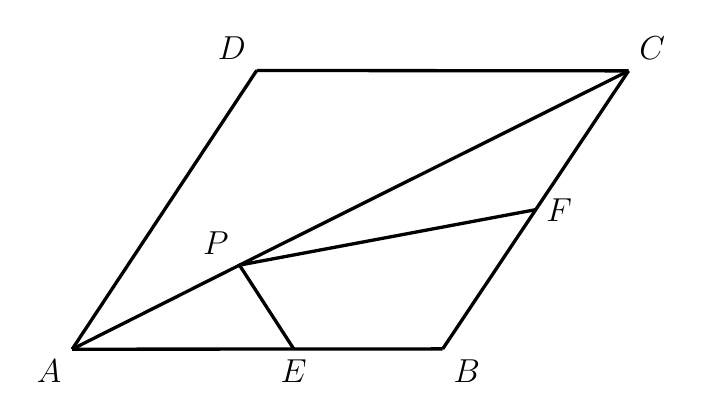
\begin{tikzpicture}[line width=1.2pt, line join=round]
\coordinate (A) at (-3.540,-1.757);
\coordinate (B) at (1.166,-1.753);
\coordinate (C) at (3.526,1.778);
\coordinate (D) at (-1.196,1.783);
\coordinate (F) at (2.345,0.015);
\coordinate (P) at (-1.415,-0.689);



\coordinate (E) at (-0.726,-1.753);


\draw (A) -- (B);
\draw (B) -- (C);
\draw (C) -- (D);
\draw (D) -- (A);
\draw (A) -- (P) -- (C);   
\draw (P) -- (F);
\draw (P) -- (E);


\node[below left]  at (A) {\fontsize{12}{14.4}\selectfont$A$};
\node[below right] at (B) {\fontsize{12}{14.4}\selectfont$B$};
\node[above right] at (C) {\fontsize{12}{14.4}\selectfont$C$};
\node[above left]  at (D) {\fontsize{12}{14.4}\selectfont$D$};
\node[below]       at (E) {\fontsize{12}{14.4}\selectfont$E$};
\node[right]       at (F) {\fontsize{12}{14.4}\selectfont$F$};
\node[above left]  at (P) {\fontsize{12}{14.4}\selectfont$P$};
\end{tikzpicture}
\end{document}